\documentclass[accentcolor=tud4b,colorbacktitle,inverttitle,landscape,german,presentation,t]{tudbeamer}
\mathcode`\,="013B%L�scht das Leerzeichen nach dem Komma in Dezimalzahlen
%\usepackage{multimedia}

%\usepackage{media9}

%\usepackage{movie15}


\usepackage{hyperref}
\usepackage{bbding}
\usepackage{units}
\usepackage{epstopdf}
\usepackage{subfigure}
\usepackage{caption}
%\usepackage{ngerman}
\usepackage{color}
\usepackage{rotating}
\usepackage{amsmath}
\usepackage{capt-of}
\usepackage{gensymb}
\usepackage[latin1]{inputenc}   % deutsche Umlaute
\usepackage[T1]{fontenc}        % Darstellung von Schrift als echte T1 Fonts und nicht als Bilder
\usepackage{graphicx}
\usepackage{wasysym}
\graphicspath{{bilder/}}
% \usepackage{multimedia}
% \usepackage[square]{natbib}
% \usepackage{bibgerm}
\usepackage{tikz}

\usetikzlibrary{shapes.geometric,shapes.arrows,decorations.pathmorphing}
\usetikzlibrary{matrix,chains,scopes,positioning,arrows,fit}
\usetikzlibrary{calc}
\usetikzlibrary{patterns}

% \usetikzlibrary{patterns}
 \usetikzlibrary{matrix}
 \usetikzlibrary{decorations.pathmorphing}
 \usetikzlibrary{arrows,shapes.geometric} % fadings, ???
 \usepackage{fancybox}
 \usepackage{amsmath}            % Mathematik-Umgebungen
\usepackage{bm}                 % fette Mathe Buchstaben
\usepackage{amssymb}            % spezielle Mathe-Symbole


\usepackage{color}

%
% Absolute positioning
% beamer paper size: 12.80cm x 9.60cm
%
\usepackage[overlay,absolute]{textpos}
\setlength{\TPHorizModule}{10mm}
\setlength{\TPVertModule}{\TPHorizModule}
\textblockorigin{5mm}{25.5mm}
\setlength{\parindent}{0pt}

\newcommand{\leftbox}[1]{
 \begin{textblock}{5.7}(0, 0)
   #1
 \end{textblock}
}

\newcommand{\rightbox}[1]{
 \begin{textblock}{5.7}(6.1, 0)
   #1
 \end{textblock}
}

\newcommand{\fullbox}[1]{
 \begin{textblock}{11.8}(0, 0)
   #1
 \end{textblock}
}

% \usepackage{calc}
\newenvironment{arbbox}[2]
{%\setlength{\boxwidth}{11.8cm minus \real{#1}}
\begin{textblock}{11.8cm}(#1, #2)}
{\end{textblock}}




%
% Macros
%
% \renewcommand{\vec}[1]{\ensuremath{\bm{#1}}}
\renewcommand{\vec}[1]{\ensuremath{\boldsymbol{#1}}}
\newcommand*{\vpointer}{\vcenter{\scalebox{2}{\Huge\pointer}}}

\begin{document}
\title[]{Automatic distortion calibration}
\subtitle{Ahmed Ashraf, Nils Hamacher, Linghan Qian, Vivica Wirth}

\author[Gruppe Acu\~na]{Gruppe Acu\~na}
\institute[Regelungsmethoden und Robotik | Projektseminar Robotik]{Regelungsmethoden und Robotik | Projektseminar Robotik}




% \logo{\color{tudtextaccent}TU Darmstadt-}
\logo{
\includegraphics{rmr2}}

\date{15.07.2017}
%Titelfolie%%%%%%%%%%%%%%%%%%%%%%%%%%%%%%%%%%%%%%%%%%%%%%%%%%%%%%%%%%%%%%%%%%%%%%%%%%%%%%%%%%%%%%%%%%%%%%%%%%%%%%%%%%%%%%%%%%%%%%%%%%%%%%%%%%%%%%%%%%%%%%%%%%%
\begin{titleframe}
\leftbox{
\begin{center}
\vspace{1.2cm}
\begin{figure}
\includegraphics[width=5.2cm]{distortedImage}
\end{figure}
\end{center}
}

\begin{center}
\vspace{2.3cm}
$\vpointer$
\end{center}

\rightbox{
\vspace{1.2cm}
\begin{center}
\begin{figure}
\includegraphics[width=5.2cm]{mappedImage}
\end{figure}
\end{center}
}

\end{titleframe}

%Hauptfolien%%%%%%%%%%%%%%%%%%%%%%%%%%%%%%%%%%%%%%%%%%%%%%%%%%%%%%%%%%%%%%%%%%%%%%%%%%%%%%%%%%%%%%%%%%%%%%%%%%%%%%%%%%%%%%%%%%%%%%%%%%%%%%%%%%%%%%%%%%%%%%%%%%%
%%%%%%%%%%
\begin{frame}{\\Task description\\} \leftbox{
 \vspace{0.5cm}
 \begin{figure} 
 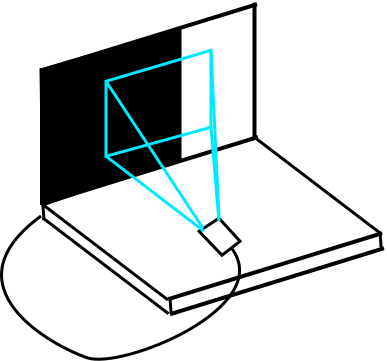
\includegraphics[scale=0.15]{rect}
 \caption{System}%source
 \end{figure}
 }
 \rightbox{
 \vspace{1cm}
\textbf{Task:} \\
Calibrate camera distortion automatically\\
\textbf{Advantage:}\\
\textbf{Efficiency}\\
No human-interaction\\

\textbf{Dense model}\\
1.	Precise position	\\	
2.	Non-parametric \\
 }
\end{frame}


\begin{frame}{\\Distortion example\\ \small{Source \cite{Villiers}}}

 \vspace{-1cm}
 \begin{align*}
 x &=x_d+ (x_d-x_c)(1+K_1r^2+K_2r^4)+P_1\left( r^2+2(x_d-x_c)^2\right) +2P_2(x_d-x_c)(y_d-y_c)\\
 y &= y_d+(y_d-y_c)(1+K_1r^2+K_2r^4)+2P_1(x_d-x_c)(y_d-y_c)+P_2\left(r^2+2((y_d-y_c)^2\right) 
 \end{align*}

 \leftbox{
 \vspace{2cm}
 \textbf{Radial distortion:}
 \begin{align*}
 K_n = n^{th} \text{ radial distortion coefficient}
 \end{align*}
}
\rightbox{
 \vspace{2cm}
 \textbf{Tangential distortion:}
  \begin{align*}
 P_n = n^{th}~\text{tangential distortion coefficient}
 \end{align*}

}
\vspace{2cm}
\begin{align*}
(x_d,~y_d) = ~&\text{distorted image point as projected on image plane,}\\
(x,~y) =~&\text{undistorted image point as projected on image plane,}\\
(x_c,~y_c) =~&\text{distortion center,}\\
r =~&\sqrt{(x_d-x_c)^2+(y_d-y_c)^2},\\
 &\text{coefficients bigger $2$ were not considered.}
\end{align*}
\end{frame}



\begin{frame}{\\Distortion example}

 \vspace{-1cm}
 \begin{align*}
 x &=x_d+ (x_d-x_c)(1+K_1r^2+K_2r^4)+P_1\left( r^2+2(x_d-x_c)^2\right) +2P_2(x_d-x_c)(y_d-y_c)\\
 y &= y_d+(y_d-y_c)(1+K_1r^2+K_2r^4)+2P_1(x_d-x_c)(y_d-y_c)+P_2\left(r^2+2((y_d-y_c)^2\right)
 \end{align*}


 \leftbox{
 \vspace{1.5cm}
 \textbf{Radial distortion:}
 \begin{figure}
 \includegraphics[scale=0.3]{distortions_inline}
 \caption{radial distortions \cite{Mannuru}}%source
 \end{figure}
}
\rightbox{
 \vspace{1.5cm}
\textbf{Tangential distortion:}
 \begin{figure}
 \includegraphics[scale=0.275]{tangential_dist}
 \caption{first order tangential distortion \cite{Ribbens}}%source
 \end{figure}

}

\end{frame}



\begin{frame}{\\Applying directional filters to extract edges\\ \small{Sobel operator}}

\begin{columns}
\column{0.35\textwidth}
\vspace{-1cm}
\begin{figure}
\includegraphics[scale=.385]{Sobel_1}
\caption{Original image \cite{youtube} }
\end{figure}



\column{0.35\textwidth}
\vspace{-1cm}
\begin{figure}
\includegraphics[scale=.58]{Sobel_4_y}
\caption{Vertical edges \cite{youtube} }
\end{figure}

\column{0.35\textwidth}
\vspace{-1cm}

\begin{figure}
\includegraphics[scale=.6]{Sobel_4_x}
\caption{Horizontal edges \cite{youtube} }
\end{figure}
\end{columns}

\rightbox{
\vspace{4.6 cm}
$$Kernel_{horizontal}= Kernel_{vertical}^T$$
}
\leftbox{
\vspace{4.25cm}
$$Kernel_{vertical}=\begin{pmatrix}
-1&0&1\\-2&0&2\\-1&0&1\\\end{pmatrix}$$
}
\end{frame}

\begin{frame}{\\Applying directional filters to extract edges\\ \small{Canny operator}}
\begin{columns}

\column{0.5\textwidth}
\vspace{-1cm}
\begin{figure}
\includegraphics[scale=.5]{Sobel_3}
\caption{Orientation image \cite{youtube} }
\end{figure}
$$|grad(I)|=\sqrt[2]{\left(\frac{\partial I}{\partial x}\right)^2+\left(\frac{\partial I}{\partial y}\right)^2}$$

\column{0.5\textwidth}
\vspace{-.15cm}
\begin{figure}
\includegraphics[scale=.35]{Canny_2}
\caption{Canny image }
\end{figure}

$$\theta_{orientation}=\arctan{\left(\frac{\partial I}{\partial y},\frac{\partial I}{\partial x}\right)}$$

\end{columns}
\end{frame}

\begin{frame}{\\Applying directional filters to extract edges\\ \small{Algorithms comparison \cite{youtube}}}

\begin{columns}

\column{0.35\textwidth}
\textbf{Original image}
\begin{figure}
\includegraphics[scale=.45]{Sobel_1}
\caption{Original image}
\end{figure}

\column{0.35\textwidth}
\textbf{Sobel operator}
\begin{figure}
\includegraphics[scale=.45]{Sobel_2}
\caption{Image with Sobel operator }
\end{figure}
\column{0.3\textwidth}
\textbf{Canny operator}
\vspace{1.2cm}
\begin{figure}
\includegraphics[scale=.22]{Canny_2}
\caption{Image with Canny operator }
\end{figure}

\end{columns}


\end{frame}


\begin{frame}{\\pixel size detection}

%\vspace{4cm}
\leftbox{
 %\vspace{2cm}
 \textbf{pixelSize = 1:}
 \begin{figure}
 \includegraphics[scale=0.1]{pixelSizeImg1}
  \end{figure}
}
\rightbox{
 %\vspace{2cm}
\textbf{pixelSize = 8:}
 \begin{figure}
 \includegraphics[scale=0.1]{pixelSizeImg2}
 \end{figure}

}
 
\end{frame}

\begin{frame}{\\Center point estimation}

 \begin{figure}
 \vspace{-0.5cm}
 \includegraphics[scale=0.15]{pixelSizeImg2_FOV}
 \end{figure}
 \leftbox{
  \vspace{4.5cm}
  \begin{align*}
  \textbf{x}_c =\frac{\sum\limits_{k=1}^{n} \textbf{x}_k}{n}
  \end{align*}
 }
 \rightbox{
  \vspace{5cm}
  %\begin{align*}
  $n$~~~:~number of seen pixels\\
  $\textbf{x}_k$~:~position of seen pixel
  %\end{align*}
}
\end{frame}






\begin{frame}{\\Runtime}
\begin{itemize}
\item Map gaining:\begin{itemize}
\item Depends on approach used
\item Usual dependencies
\begin{itemize}
\item \#~images
\item Field of View (FOV)
\item Turnover rate of images (3 images per seconds)
\item Framerate (21 frames per second)
\end{itemize}
\end{itemize}
\item Interpolate Map $<100~ms$
\item Correct distortion $<100~ms$
\end{itemize}

\end{frame}

\begin{frame}{\\Runtime\\ \small{FOV}}
\begin{figure}
\vspace{-0.5cm}
\hspace{2cm}
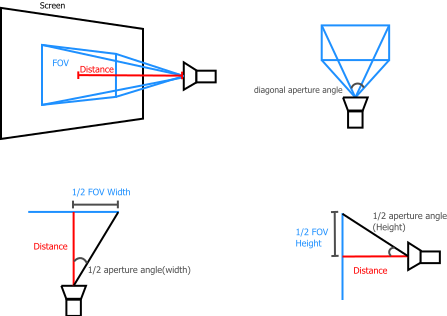
\includegraphics[scale=0.35]{distanceandangles}
\end{figure}
\vspace{-5.5cm}
\textbf{Received Info:}
\begin{itemize}
\item $\alpha_{width||height}$
\item $\alpha_{diag}$
\end{itemize}
\vspace{1cm}
\textbf{Our FOV:}
\begin{itemize}
\item $670$x$395$ pixels
\item $\alpha_{diag} = 68.46\degree$
\item camera specs:\\$\alpha_{diag,s} = 68.5\degree$
\end{itemize}
\end{frame}

%\begin{frame}{\\Runtime\\ \small{Pixelwise}}

%\textbf{Naive:}
%\begin{align*}
%rt(w_s,h_s) = \frac{1}{3}w_s\cdot h_s =307,200sec
%\end{align*}

%\textbf{Spiral:}
%\begin{align*}
%rt(w_{FOV},h_{FOV}) = \frac{1}{3}(w_{FOV}+1)\cdot (h_{FOV}+1)=88,572sec
%\end{align*}
%\leftbox{
%\vspace{4cm}
%\begin{align*}
%w_s~&:~\text{width of screen}\\
%h_s~&:~\text{height of screen}
%\end{align*}
%}
%\rightbox{
%\vspace{4cm}
%\begin{align*}
%w_{FOV}~&:~\text{wdith of FOV}\\
%h_{FOV}~&:~\text{height of FOV}
%\end{align*}

%}
%\end{frame}


\begin{frame}{\\Runtime\\ \small{Line-based}}

\textbf{naive:}
\begin{align*}
rt(w_s,h_s) = \frac{1}{3}(w_s+ h_s) =790sec
\end{align*}
\leftbox{\vspace{2cm}
\begin{align*}
w_s~&:~\text{width of screen}\\
h_s~&:~\text{height of screen}
\end{align*}}
\rightbox{\vspace{2cm}
\begin{align*}
w_{FOV}~&:~\text{wdith of FOV}\\
h_{FOV}~&:~\text{height of FOV}
\end{align*}}
\end{frame}


\begin{frame}{\\Runtime\\ \small{Line-based}}
Center point \& FOV based:
\begin{itemize}\vspace{0.5cm}
\item[1.] $rt_{cp}(w_s,h_s,s) = \frac{w_s\cdot h_s}{3s^2}$\vspace{0.5cm}
\item[2.] $rt_{map}(w_{FOV},h_{FOV},s,m,j) = \frac{1}{3j}\left(w_{FOV}+2s+2m+h_{FOV}+2s+2m\right)$\vspace{0.5cm}
\item[3.] $rt\left( w_s,h_s,w_{FOV},h_{FOV},s,m,j\right) = \frac{1}{3}\left((w_{FOV}+4s+4m+h_{FOV})\frac{1}{j}+ \frac{w_s\cdot h_s}{s^2}\right)$
\end{itemize}

\vspace{0.5cm}
\small{ $s$~~: space between lit pixels in center point estimation\\ $m$ : safety margin\\ $j$~~~: skip range}

\end{frame}


\begin{frame}{\\Runtime\\ \small{Line-based}}
\textbf{Find optimum}\\

\begin{align*}\hspace{-1cm}
rt'(s)&= -\frac{w_s h_s}{3s^3}+\frac{4}{3j} \stackrel{!}{=} 0\\
\vspace{0.5cm}
s &= \sqrt[3]{\frac{w_s\cdot h_s\cdot j}{4}}
\end{align*} 

\vspace{0.5cm}
For our Setup
\leftbox{\vspace{3.5cm}
\vspace{1cm}
\textbf{$j=1$:}\\
$s=70 \hspace{0.5cm}\Rightarrow \hspace{0.5cm} rt = 550$\\
}
\
\rightbox{\vspace{4.5cm}
\textbf{$j=3$:}\\
$s=101 \hspace{0.5cm}\Rightarrow \hspace{0.5cm} rt = 211$\\  %(1920,1080,670,395,70,5,3)
}

\end{frame}



\begin{frame}{\\Overview implementation\\ \small{UML diagramm}}
\begin{figure}
\hspace{-0.50cm}
\includegraphics[scale=0.275]{uml_diagram}
\caption{overview of classes, structs, and namespaces}

\end{figure}

\end{frame}

\begin{frame}{\\Results}
\leftbox{
 %\vspace{2cm}
 \textbf{Ground truth:}
 \begin{figure}
 \includegraphics[scale=0.2]{gt}
 \caption{all white lines in FOV}
  \end{figure}
}
\rightbox{
 %\vspace{2cm}
\textbf{Mapped Image: }
 \begin{figure}
 \includegraphics[scale=0.2]{mappedImage}
 \caption{the seen lines after they were mapped by the algorithm}
 \end{figure}
 }
\end{frame}

\begin{frame}{\\Comparison\\ \small{Subtraction of ground truth and mapped image}}
\begin{figure}
\vspace{-0.5cm}
\includegraphics[scale=0.35]{substracted}
\caption{difference of both images\\ $2,983$ of $333,756$ pixels ($0.89\%$) do not fit}
\end{figure}

\end{frame}

\begin{frame}{\\Future Work}
\begin{itemize}
\item Run mapping in one step with \emph{openframeworks}-version
\item detect white threshold
\item improvement of line detection $\Rightarrow$ line counting?
\item avoid implausible mapping
\item undo statemachine, if internal \emph{openframeworks}-timing works
\end{itemize}

\end{frame}


\begin{frame}{\\ The End}
\begin{center}
\vspace{1.5 cm}
Thank you all for your attention!\\
Are there any questions?
\end{center}
\end{frame}


\begin{frame}{\\Sources}
\begin{thebibliography}{1}
\bibitem {youtube}
Computerphile \\
\url {https://www.youtube.com/watch?v=uihBwtPIBxM}
15.07.2017.\\
\url {https://www.youtube.com/watch?v=sRFM5IEqR2w}
15.07.2017.
\bibitem{Ribbens}
B.~Ribbens, V.A.~ Jacobs, C.~Vuye1, J.A.N.~Buytaert, J.J.J.~ Dirckx, and S.~Vanlanduit. \emph{High-resolution temporal profilometry using Fourier estimation}, 2007
\bibitem{Mannuru}
S.~Mannuru. \emph{A fully automated geometric lens distortion correction method}, University of Dayton, Ohio 2011
\bibitem{Villiers}
J.~P.~de ~Villiers, F.W.~Leuschnerb, R.~Geldenhuys. \emph{Centi-pixel accurate real-time inverse distortion corretion}, University of Pretoria, South Africa 2008
\end{thebibliography}
\end{frame}

\end{document}
%% High-resolution temporal profilometry using Fourier estimation (PDF Download Available). Available from: https://www.researchgate.net/publication/236330080_High-resolution_temporal_profilometry_using_Fourier_estimation [accessed Jul 16, 2017] Source image tangential dist